% Mobile-C Library 

%%%%%%%%%%%%%%%%%%%%%%%%%%%%%%%%%%%%%%%%%%%%%%%%%%%%%%%%%%%%%%%%%%%%%%
% Preamble {{{
%\documentclass[11pt]{article}
\documentclass[11pt]{report}
\usepackage{varioref}
\usepackage{times,verbatim,fancyheadings,makeidx}
\usepackage{moreverb}
%\usepackage{psfig}
\usepackage[pdftex]{hyperref}
\usepackage{hypcap}
\usepackage{fullpage}
\usepackage{amssymb,amsmath}
\usepackage{graphicx}
\usepackage{program}
%\headrulewidth 0.0pt
%\hoffset=-0.0625in
%\voffset=0pt
\setlength{\textheight}{9in}
\setlength{\textwidth}{6.5in}
\topmargin=0.05in
\makeindex
% }}} Preamble
%%%%%%%%%%%%%%%%%%%%%%%%%%%%%%%%%%%%%%%%%%%%%%%%%%%%%%%%%%%%%%%%%%%%%%

%%%%%%%%%%%%%%%%%%%%%%%%%%%%%%%%%%%%%%%%%%%%%%%%%%%%%%%%%%%%%%%%%%%%%%
% Title Page {{{
\begin{document}
\thispagestyle{empty}
\begin{center}
%\includegraphics[width=1.8in]{figure/mobilec_logo.png}


\vspace{0.5in}
{\Huge\sf\bf User's Guide for Programming iMobot} \\
\vspace{2.0in}
{\large\sf\bf\today}
%September 20, 2007
\end{center}

\pagebreak
% }}} Title Page
%%%%%%%%%%%%%%%%%%%%%%%%%%%%%%%%%%%%%%%%%%%%%%%%%%%%%%%%%%%%%%%%%%%%%%

%%%%%%%%%%%%%%%%%%%%%%%%%%%%%%%%%%%%%%%%%%%%%%%%%%%%%%%%%%%%%%%%%%%%%%
% Abstract {{{
%\phantomsection
%\addcontentsline{toc}{chapter}{Abstract}
\begin{abstract} 
This user's guide describes how to control an iMobot robotic module.

\end{abstract}
\pagebreak
% Abstract }}}
%%%%%%%%%%%%%%%%%%%%%%%%%%%%%%%%%%%%%%%%%%%%%%%%%%%%%%%%%%%%%%%%%%%%%%

%%%%%%%%%%%%%%%%%%%%%%%%%%%%%%%%%%%%%%%%%%%%%%%%%%%%%%%%%%%%%%%%%%%%%%
% Table of Contents {{{
\pagenumbering{roman}
\setcounter{page}{1}
\tableofcontents
\pagebreak
% }}} Table of Contents
%%%%%%%%%%%%%%%%%%%%%%%%%%%%%%%%%%%%%%%%%%%%%%%%%%%%%%%%%%%%%%%%%%%%%%

%%%%%%%%%%%%%%%%%%%%%%%%%%%%%%%%%%%%%%%%%%%%%%%%%%%%%%%%%%%%%%%%%%%%%%
% Part 1 {{{
\pagenumbering{arabic}
\setcounter{page}{1}
\pagebreak
% }}} Part 1 
%%%%%%%%%%%%%%%%%%%%%%%%%%%%%%%%%%%%%%%%%%%%%%%%%%%%%%%%%%%%%%%%%%%%%%

%%%%%%%%%%%%%%%%%%%%%%%%%%%%%%%%%%%%%%%%%%%%%%%%%%%%%%%%%%%%%%%%%%%%%%
% Introduction {{{
%\pagenumbering{arabic}
%\setcounter{page}{1}
%\pagestyle{fancy}
%\chapter{Introduction}
%\pagebreak
% }}} Introduction
%%%%%%%%%%%%%%%%%%%%%%%%%%%%%%%%%%%%%%%%%%%%%%%%%%%%%%%%%%%%%%%%%%%%%%

\chapter{Getting Started}
This short guide will enable you to run the provided demo program,
``simple.cpp'', on the iMobot.
\begin{enumerate}
\item Download and install a VNC client
  \begin{itemize}
  \item For Windows, you may download and install TightVNC from \texttt{http://www.tightvnc.com}.
  \item For Mac OS X, you may download and install Chicken of the VNC from\\
  \texttt{http://sourceforge.net/projects/cotvnc/}
  \end{itemize}
\item Log in to the imobot with a VNC client. 
\item Connect to the iMobot with your VNC client. The iMobot will create an ad-hoc network
called "imobot" by default upon startup. Connect to the ad-hoc network, and connect
to the iMobot's IP address, which is 192.168.0.1 by default.
\item Open and execute the demo program.
  \begin{enumerate}
  \item Copy the demo program to your home directory with the command\\
  \texttt{cp /usr/local/ch/package/chimobot/demos/simple.cpp \textasciitilde/}
  \item Open the demo program with ChIDE. You may left click on the desktop to open the menu, and select \texttt{Applications -> Accessories -> ChIDE}.
  \item Click on \texttt{File -> Open} within ChIDE and open the program, \texttt{simple.cpp}. 
  \item Click on the ``Run'' button, located near the top right of the ChIDE Window. The robot should now run the program.
  \end{enumerate}
\end{enumerate}

\chapter{Graphical Control Interface}
\begin{figure}
\begin{center}
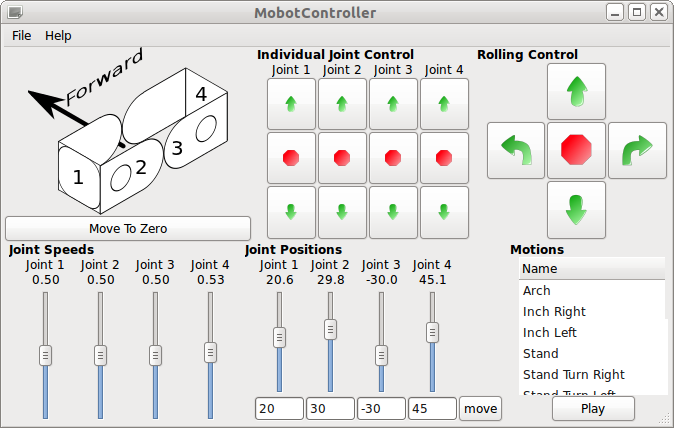
\includegraphics[width=4in]{gui_screenshot.png}
\caption{\label{fig:gui}The iMobot Graphical Control Interface.}
\end{center}
\end{figure}
The iMobot comes with a graphical control interface for controlling the iMobot.
The control interface is able to perform simple locomotion tasks, and can be
used to determine the joint angles of the iMobot. A screenshot of the interface
is shown in Figure \ref{fig:gui}.

The graphical interface can be found in the application menu of the iMobot. Once
a VNC connection to the iMobot has been established, simply left click on the
desktop to bring up the menu, and select the item \texttt{Applications ->
Accessories -> iMobot Controller}. Once the controller starts, it needs to be
initialized in order to establish communication with the motor controllers.
This is done by clicking on \texttt{File -> Init Local I2C Bus}. Ensure that 
the application is connected by ensuring that the status bar at the bottom of the
application displays ``Connected''. 

The graphical interface is composed of six basic components, as shown in
Figure \ref{fig:gui}. There are three components on the top half of the
interface, and three on the bottom half. Each component is discussed in
detail in the following subsections.

\subsection{The iMobot Diagram and ``Move To Zero'' Button}
The first section of the GUI located on the top left of the interface
displays a schematic diagram of the iMobot, displaying motor positions.
Underneath the diagram, there is a large button with the text 
``Move To Zero''. When clicked, this button will command the connected
iMobot to rotate all of its joints to a flat ``Zero'' position.

\subsection{Individual Joint Control}
The second section, located at the top-middle section of the interface,
is the ``Individual Joint Control'' section. These buttons command the
iMobot to move individual joints. When the up or down arrows are clicked,
the iMobot begins to move the corresponding joint in either the positive,
or negative direction. The joint will continue to move until the stop 
button, located between the up and down arrows, is clicked. 

\subsection{Rolling Control}
This section contains buttons for controlling the iMobot as a 
two wheeled mobile robot. The up and down buttons cause the iMobot to
roll forward or backward. The left and right buttons cause the iMobot 
to rotate towards the left, or towards the right. The stop button in the
middle causes the iMobot to stop where it is.

\subsection{Joint Speeds}
The ``Joint Speeds'' section, located at the bottom left of the interface,
displays and controls the current joint speeds of the iMobot. Joint speeds
are a value between 0 and 1, with 1 meaning maximum joint power, and 0
meaning zero joint power. The speed may be set by sliding the vertical 
sliders to the desired positions. 

\subsection{Joint Positions}
This section, located in the bottom-middle of the interface, is used to display
and control the positions of each of the four
joints of a iMobot. The joint positions are displayed in the numerical
text located above each vertical slider. The displayed joint positions are in
units of degrees.  There are two methods to control
the joints using this interface.

The first method of controlling the joints is by using the vertical sliders.
Each vertical slider's position represents a joint's angle. The sliders for the
two end joints vary from -180 degrees to 180 degrees, representing one complete
rotation. The angles for the two body joints vary from -90 to 90 degrees. When
the position of the slider is moved, the iMobot will move its joints to match the 
sliders. 

The second method for moving the joints is by entering the exact angles for the
joints. Below each of the four sliders lies a text entry box. Values in degrees
may be typed into each of the four entry boxes. When the button on the lower
right of the section labeled ``Move'' is clicked, the iMobot will move its joints
to match the values typed into the boxes. If no value is typed into a box, that 
joint will not move.

\subsection{Motions}
This section, located on the bottom right of the interface, contains a set of
preprogrammed motions for the iMobot. To execute a preprogrammed motion, simply
click on the name of the motion you wish to execute, and then click the button
labeled ``Play''.


%%%%%%%%%%%%%%%%%%%%%%%%%%%%%%%%%%%%%%%%%%%%%%%%%%%%%%%%%%%%%%%%%%%%%%
% SUB: Overview of Sample Application Programs {{{
\chapter{Overview of Sample Application Programs}
\subsection{\texttt{simple.cpp} : A Simple Bare-Bones Demo}
The following program is a simple program which moves some joints on the iMobot
before initializing the robot to listen for incoming Bluetooth commands.
\subsubsection{simple.cpp \label{subsec:simple.cpp}}
\listinginput{1}{../demos/simple_cpp/simple.cpp}
\subsubsection{Explanation of simple.cpp}
\begin{itemize}
\item 
\begin{verbatim}
  CiMobot robot;
\end{verbatim}
This line declares the \texttt{robot} object, which represents the
capabilities of the iMobot module. iMobot modules are represented by
the \texttt{CiMobot} type. This object contains various member
functions which may be executed by the user.
\item 
\begin{verbatim}
  robot.moveToZero();
\end{verbatim}
These commands command the iMobot to move all motors to their zero positions
and wait until the motion is finished.
\item 
\begin{verbatim}
  robot.moveTo(90, 0, 0, 90);
\end{verbatim}
These lines instruct the robot to rotate the faceplates, which are the first
and fourth joints, by 90 degrees. 
\item 
\begin{verbatim}
  robot.moveTo(0, 0, 0, 0);
\end{verbatim}
The previous line causes the iMobot to move the first and fourth joints back to
their original position.
\end{itemize}

\subsection{\texttt{bluetoothListener.cpp} : A Demo That Receives and Executes
Bluetooth Commands}
The following program is a bare-bones demo program which initializes the iMobot's
Bluetooth listening capabilities. The program sets up the iMobot so that Bluetooth
enabled devices can connect to and control the iMobot remotely. 
\subsubsection{bluetoothListener.cpp}
\listinginput{1}{../demos/bluetoothListener/bluetoothListener.cpp}
\subsubsection{Explanation of \texttt{bluetoothListener.cpp}}
\begin{itemize}
\item 
\begin{verbatim}
  CiMobot robot;
  int bluetoothChannel = 20; // Default channel
\end{verbatim}
Similar to the previous demo, the first line declares a \texttt{CiMobot} object
called \texttt{robot}. The second line declares an integer variables called 
\texttt{bluetoothChannel}, which is initialized to a value of 20. The 
variable \texttt{bluetoothChannel} represents the channel to listen on
for incoming bluetooth connections.
\item
\begin{verbatim}
  robot.setJointSpeed(IMOBOT_JOINT1, 0.50);
  robot.setJointSpeed(IMOBOT_JOINT2, 0.50);
  robot.setJointSpeed(IMOBOT_JOINT3, 0.50);
  robot.setJointSpeed(IMOBOT_JOINT4, 0.50);
\end{verbatim}
These lines of code set the motor speeds for all four motors to a value of
\texttt{0.50}, or 50\% speed.
\item
\begin{verbatim}
  robot.initListenerBluetooth(bluetoothChannel);
\end{verbatim}
This line initializes the iMobot's Bluetooth listening service. 
\item
\begin{verbatim}
  robot.listenerMainLoop();
\end{verbatim}
This function blocks indefinitely, allowing the iMobot to handle any number of Bluetooth
commands from the remote device. The \texttt{listenerMainLoop()} will return if the
``Quit'' command is sent to the iMobot from the remote device.
\end{itemize}

This demo enables an iMobot to accept bluetooth connections from the corresponding
MoBot library, called \texttt{CMobot}. Please refer to the MoBot documentation
for instructions on how to connect to and control a MoBot remotely via Bluetooth.

%%%%%%%%%%%%%%%%%%%%%%%%%%%%%%%%%%%%%%%%%%%%%%%%%%%%%%%%%%%%%%%%%%%%%%
% SUB: Execution of Sample Applications {{{
%\section{Execution of Sample Applications}
%%%%%%%%%%%%%%%%%%%%%%%%%%%%%%%%%%%%%%%%%%%%%%%%%%%%%%%%%%%%%%%%%%%%%%
% Appendix {{{
\appendix
\chapter{Data Types, Macros, and Constants}
\section{Data Types}
There are data types which are used by the MoBot library to represent 
certain values, such as joint id's and motor directions.

\begin{tabular}{p{3.5cm}p{7cm}} \hline 
Data Type& Description \\
\hline 
\texttt{mobotJointId\_t} & An enumerated value that indicates a MoBot joint. \\
\texttt{mobotJointState\_t} & The current state of a MoBot joint. \\
\texttt{mobotJointDirection\_t} & The current motion direction of a MoBot joint. 
\end{tabular}

\subsection{\label{sec:mobotJointId_t}\texttt{mobotJointId\_t}}
This datatype is an enumerated type used to identify a joint on the MoBot. Valid
values for this type are:
\begin{verbatim}
typedef enum mobot_joints_e {
  MOBOT_JOINT1 = 1,
  MOBOT_JOINT2 = 2,
  MOBOT_JOINT3 = 3,
  MOBOT_JOINT4 = 4
} mobotJointId_t;
\end{verbatim}
The joints are enumerated in order from one side of the MoBot to the other. Joints 1 and 4
are faceplate joints, and joints 2 and 3 are body joints.

\subsection{\label{sec:mobotJointState_t}\texttt{mobotJointState\_t}}
This datatype is an enumerated type used to designate the current 
movement state of a joint. Valid values are:
\begin{itemize}
\item \texttt{MOBOT\_JOINT\_IDLE}: This value indicates that the joint is not moving.
\item \texttt{MOBOT\_JOINT\_MOVING}: This value indicates that the joint is currently moving.
\item \texttt{MOBOT\_JOINT\_GOALSEEK}: This value indicates that the joint is currently moving
  towards a predefined goal.
\end{itemize}

\subsection{\label{sec:mobotJointDirection_t}\texttt{mobotJointDirection\_t}}
This datatype designates a MoBot joint's commanded direction of travel. Valid values
are
\begin{itemize}
\item \texttt{MOBOT\_NEUTRAL}: There is no predesignated direction for the
joint. If the joint is commanded to move to a specific location, the MoBot will
decide the best direction to move the joint in order to achieve the goal with
the smallest motion.
\item \texttt{MOBOT\_FORWARD}: Move the joint in the direction which increases its 
angular position.
\item \texttt{MOBOT\_BACKWARD}: Move the joint in the direction which decreases
its angular position.
\end{itemize}

\section{Macros}

\subsection{\texttt{MoBot\_joints\_t}}
\index{MoBot\_joints\_t}
The data type \texttt{MoBot\_joints\_t} contains the following macro datatypes.\\

\index{IMOBOT\_JOINT1}
\index{IMOBOT\_JOINT2}
\index{IMOBOT\_JOINT3}
\index{IMOBOT\_JOINT4}
\begin{tabular}{p{3cm}p{7cm}} \hline 
Value & Description \\
\hline 
\texttt{IMOBOT\_JOINT1} & Joint number 1 on the MoBot, which is a faceplate joint. \\
\texttt{IMOBOT\_JOINT2} & Joint number 2 on the MoBot, which is a body joint. \\
\texttt{IMOBOT\_JOINT3} & Joint number 3 on the MoBot, which is a body joint. \\
\texttt{IMOBOT\_JOINT3} & Joint number 4 on the MoBot, which is a faceplate joint. 
\end{tabular}

\subsection{\texttt{MoBot\_joint\_direction\_t}}
\index{MoBot\_joint\_direction\_t}
The data type \texttt{MoBot\_joint\_direction\_t} indicates the commanded direction 
of a joint on the MoBot.

\index{IMOBOT\_NEUTRAL}
\index{IMOBOT\_FORWARD}
\index{IMOBOT\_BACKWARD}
\begin{tabular}{p{3cm}p{7cm}} \hline 
Value & Description \\
\hline 
\texttt{IMOBOT\_NEUTRAL} & This value indicates automatic direction control for a joint. 
The MoBot will choose the best direction to attain the commanded joint position. \\
\texttt{IMOBOT\_FORWARD} & Move the joint in the forward direction. \\
\texttt{IMOBOT\_BACKWARD} & Move the joint in the backward direction. \\
\end{tabular}

\chapter{iMobot API}
% Mobile-C Library 

%%%%%%%%%%%%%%%%%%%%%%%%%%%%%%%%%%%%%%%%%%%%%%%%%%%%%%%%%%%%%%%%%%%%%%
% Preamble {{{
%\documentclass[11pt]{article}
\documentclass[11pt]{report}
\usepackage{varioref}
\usepackage{times,verbatim,fancyheadings,makeidx}
\usepackage{moreverb}
%\usepackage{psfig}
\usepackage[pdftex]{hyperref}
\usepackage{hypcap}
\usepackage{fullpage}
\usepackage{amssymb,amsmath}
\usepackage{graphicx}
\usepackage{program}
%\headrulewidth 0.0pt
%\hoffset=-0.0625in
%\voffset=0pt
\setlength{\textheight}{9in}
\setlength{\textwidth}{6.5in}
\topmargin=0.05in
\makeindex
% }}} Preamble
%%%%%%%%%%%%%%%%%%%%%%%%%%%%%%%%%%%%%%%%%%%%%%%%%%%%%%%%%%%%%%%%%%%%%%

%%%%%%%%%%%%%%%%%%%%%%%%%%%%%%%%%%%%%%%%%%%%%%%%%%%%%%%%%%%%%%%%%%%%%%
% Title Page {{{
\begin{document}
\thispagestyle{empty}
\begin{center}
%\includegraphics[width=1.8in]{figure/mobilec_logo.png}


\vspace{0.5in}
{\Huge\sf\bf User's Guide for Programming iMobot} \\
\vspace{2.0in}
{\large\sf\bf\today}
%September 20, 2007
\end{center}

\pagebreak
% }}} Title Page
%%%%%%%%%%%%%%%%%%%%%%%%%%%%%%%%%%%%%%%%%%%%%%%%%%%%%%%%%%%%%%%%%%%%%%

%%%%%%%%%%%%%%%%%%%%%%%%%%%%%%%%%%%%%%%%%%%%%%%%%%%%%%%%%%%%%%%%%%%%%%
% Abstract {{{
%\phantomsection
%\addcontentsline{toc}{chapter}{Abstract}
\begin{abstract} 
This library implements control functions for controlling an iMobot
robotic module.

\end{abstract}
\pagebreak
% Abstract }}}
%%%%%%%%%%%%%%%%%%%%%%%%%%%%%%%%%%%%%%%%%%%%%%%%%%%%%%%%%%%%%%%%%%%%%%

%%%%%%%%%%%%%%%%%%%%%%%%%%%%%%%%%%%%%%%%%%%%%%%%%%%%%%%%%%%%%%%%%%%%%%
% Table of Contents {{{
\pagenumbering{roman}
\setcounter{page}{1}
\tableofcontents
\pagebreak
% }}} Table of Contents
%%%%%%%%%%%%%%%%%%%%%%%%%%%%%%%%%%%%%%%%%%%%%%%%%%%%%%%%%%%%%%%%%%%%%%

%%%%%%%%%%%%%%%%%%%%%%%%%%%%%%%%%%%%%%%%%%%%%%%%%%%%%%%%%%%%%%%%%%%%%%
% Part 1 {{{
\pagenumbering{arabic}
\setcounter{page}{1}
\pagebreak
% }}} Part 1 
%%%%%%%%%%%%%%%%%%%%%%%%%%%%%%%%%%%%%%%%%%%%%%%%%%%%%%%%%%%%%%%%%%%%%%

%%%%%%%%%%%%%%%%%%%%%%%%%%%%%%%%%%%%%%%%%%%%%%%%%%%%%%%%%%%%%%%%%%%%%%
% Introduction {{{
%\pagenumbering{arabic}
%\setcounter{page}{1}
%\pagestyle{fancy}
%\chapter{Introduction}
%\pagebreak
% }}} Introduction
%%%%%%%%%%%%%%%%%%%%%%%%%%%%%%%%%%%%%%%%%%%%%%%%%%%%%%%%%%%%%%%%%%%%%%

\chapter{Getting Started}
This short guide will enable you to run the provided demo program,
``simple.cpp'', on the iMobot.
\begin{enumerate}
\item Log in to the imobot. In order to do this, you will need a VNC client. 
  \begin{itemize}
  \item For Windows, you may download and install TightVNC from \texttt{http://www.tightvnc.com}.
  \item For Mac OS X, you may download and install Chicken of the VNC from \texttt{http://sourceforge.net/projects/cotvnc/}.
  \end{itemize}
\item Connect to the iMobot with your VNC client. The default address of the iMobot is \texttt{192.168.0.123}.
\item Copy the demo program to your home directory with the command ``\texttt{cp /usr/local/ch/package/chimobot/demos/simple.cpp ~/}''.
\item Open the demo program with ChIDE. You may left click on the desktop to open the menu, and select \texttt{Applications -> Accessories -> ChIDE}.
\item Click on \texttt{File -> Open} within ChIDE and open the program, \texttt{simple.cpp}. 
\item Click on the ``Run'' button, located near the top right of the ChIDE Window. The robot should now run the program.
\end{enumerate}

\chapter{Gtk iMobot Controller Guide}
\begin{figure}
\begin{center}
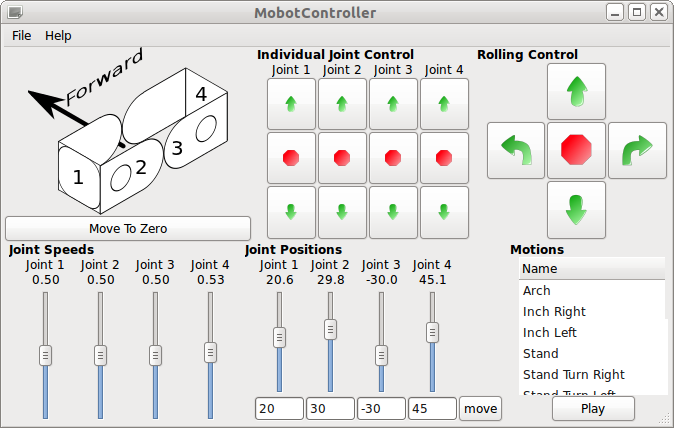
\includegraphics[width=4in]{gui_screenshot.png}
\caption{\label{fig:gui}The iMobot Graphical Control Interface.}
\end{center}
\end{figure}
The iMobot comes with a graphical control interface for controlling the iMobot.
The control interface is able to perform simple locomotion tasks, and can be
used to determine the joint angles of the iMobot. A screenshot of the interface
is shown in Figure \ref{fig:gui}.

The graphical interface can be found in the application menu of the iMobot. Once
a VNC connection to the iMobot has been established, simply left click on the
desktop to bring up the menu, and select the item \texttt{Applications ->
Accessories -> iMobot Controller}. Once the controller starts, it needs to be
initialized in order to establish communication with the motor controllers.
This is done by clicking on \texttt{File -> Init Local I2C Bus}. Ensure that 
the application is connected by ensuring that the status bar at the bottom of the
application displays ``Connected''. 

The graphical interface is composed of four basic components, as shown in
Figure \ref{fig:gui}. The first section, labeled with the red ``1'',
is a section of four sliders. Each slider controls the motor speed of a joint.

The next section, labeled ``2'', are controls which can be used to move each
joint independantly. The upward arrows indicate forward rotation, the stop
buttons stop the motors, and the downward arrows indicate backward motion.
Below the downward arrows are textboxes which display the current angle of each
joint.

The next section, labeled ``3'', contain buttons used for moving the iMobot. 
The arrows indicate forwards and backwards motion, along with turning and
sideways inchworming motions. The large stop sign button stops all motions
on the iMobot. The button labeled ``Home'' causes the iMobot to move all joints
back to their home position. 

The final section, labeled ``4'', contain preprogramed gaits for the iMobot.
To execute a gait, simply select the desired gait by left-clicking on its name,
and click the ``Play'' button.

%%%%%%%%%%%%%%%%%%%%%%%%%%%%%%%%%%%%%%%%%%%%%%%%%%%%%%%%%%%%%%%%%%%%%%
% SUB: Overview of Sample Application Programs {{{
\chapter{Overview of a Sample Application Program}
The following program is a simple program which moves some joints on the iMobot
before initializing the robot to listen for incoming Bluetooth commands.
\subsection{simple.cpp \label{subsec:simple.cpp}}
\listinginput{1}{../Demos/simple_cpp/simple.cpp}
\subsection{Explanation of simple.cpp}
\begin{itemize}
\item Lines 1-3 include the chimobot Ch package. These lines are necessary for
running Ch programs which control the iMobot. 
\item Lines 8-10 declare some local variables that are used throughout the program.
\item Line 10 declares the \texttt{robot} object, which represents the
capabilities of the iMobot module. This object contains various member
functions which may be executed by the user.
\item Lines 13-16 send commands to the iMobot to move all the joints to their
zero position.
\item Line 17 causes the program to wait until all the joints have stopped moving. 
\item Lines 20 and 21 instruct the robot to rotate joints 2 and 3 to rotate 90
degrees. Note that the joint numbers start at 0, so joints 2 and 3 are the
third and fourth joints, respectively. 
\item Lines 23 and 24 cause the program to wait until the third and fourth
joints have stopped moving.
\item Lines 26 and 27 instruct the robot to turn the third and fourth joints
back to their original zero position.
\item Lines 28 and 29 cause the program to wait until the third and fourth
joints have stopped moving.
\item Lines 33 and 34 start the Bluetooth listening service on channel 20,
which listens for Bluetooth remote commands and controls the robot accordingly. 
\item Line 37 terminates the robot control.
\end{itemize}

%%%%%%%%%%%%%%%%%%%%%%%%%%%%%%%%%%%%%%%%%%%%%%%%%%%%%%%%%%%%%%%%%%%%%%
% SUB: Execution of Sample Applications {{{
%\section{Execution of Sample Applications}
%%%%%%%%%%%%%%%%%%%%%%%%%%%%%%%%%%%%%%%%%%%%%%%%%%%%%%%%%%%%%%%%%%%%%%
% Appendix {{{
\appendix
\chapter{libimobot API}
% Mobile-C Library 

%%%%%%%%%%%%%%%%%%%%%%%%%%%%%%%%%%%%%%%%%%%%%%%%%%%%%%%%%%%%%%%%%%%%%%
% Preamble {{{
%\documentclass[11pt]{article}
\documentclass[11pt]{report}
\usepackage{varioref}
\usepackage{times,verbatim,fancyheadings,makeidx}
\usepackage{moreverb}
%\usepackage{psfig}
\usepackage[pdftex]{hyperref}
\usepackage{hypcap}
\usepackage{fullpage}
\usepackage{amssymb,amsmath}
\usepackage{graphicx}
\usepackage{program}
%\headrulewidth 0.0pt
%\hoffset=-0.0625in
%\voffset=0pt
\setlength{\textheight}{9in}
\setlength{\textwidth}{6.5in}
\topmargin=0.05in
\makeindex
% }}} Preamble
%%%%%%%%%%%%%%%%%%%%%%%%%%%%%%%%%%%%%%%%%%%%%%%%%%%%%%%%%%%%%%%%%%%%%%

%%%%%%%%%%%%%%%%%%%%%%%%%%%%%%%%%%%%%%%%%%%%%%%%%%%%%%%%%%%%%%%%%%%%%%
% Title Page {{{
\begin{document}
\thispagestyle{empty}
\begin{center}
%\includegraphics[width=1.8in]{figure/mobilec_logo.png}


\vspace{0.5in}
{\Huge\sf\bf User's Guide for Programming iMobot} \\
\vspace{2.0in}
{\large\sf\bf\today}
%September 20, 2007
\end{center}

\pagebreak
% }}} Title Page
%%%%%%%%%%%%%%%%%%%%%%%%%%%%%%%%%%%%%%%%%%%%%%%%%%%%%%%%%%%%%%%%%%%%%%

%%%%%%%%%%%%%%%%%%%%%%%%%%%%%%%%%%%%%%%%%%%%%%%%%%%%%%%%%%%%%%%%%%%%%%
% Abstract {{{
%\phantomsection
%\addcontentsline{toc}{chapter}{Abstract}
\begin{abstract} 
This library implements control functions for controlling an iMobot
robotic module.

\end{abstract}
\pagebreak
% Abstract }}}
%%%%%%%%%%%%%%%%%%%%%%%%%%%%%%%%%%%%%%%%%%%%%%%%%%%%%%%%%%%%%%%%%%%%%%

%%%%%%%%%%%%%%%%%%%%%%%%%%%%%%%%%%%%%%%%%%%%%%%%%%%%%%%%%%%%%%%%%%%%%%
% Table of Contents {{{
\pagenumbering{roman}
\setcounter{page}{1}
\tableofcontents
\pagebreak
% }}} Table of Contents
%%%%%%%%%%%%%%%%%%%%%%%%%%%%%%%%%%%%%%%%%%%%%%%%%%%%%%%%%%%%%%%%%%%%%%

%%%%%%%%%%%%%%%%%%%%%%%%%%%%%%%%%%%%%%%%%%%%%%%%%%%%%%%%%%%%%%%%%%%%%%
% Part 1 {{{
\pagenumbering{arabic}
\setcounter{page}{1}
\pagebreak
% }}} Part 1 
%%%%%%%%%%%%%%%%%%%%%%%%%%%%%%%%%%%%%%%%%%%%%%%%%%%%%%%%%%%%%%%%%%%%%%

%%%%%%%%%%%%%%%%%%%%%%%%%%%%%%%%%%%%%%%%%%%%%%%%%%%%%%%%%%%%%%%%%%%%%%
% Introduction {{{
%\pagenumbering{arabic}
%\setcounter{page}{1}
%\pagestyle{fancy}
%\chapter{Introduction}
%\pagebreak
% }}} Introduction
%%%%%%%%%%%%%%%%%%%%%%%%%%%%%%%%%%%%%%%%%%%%%%%%%%%%%%%%%%%%%%%%%%%%%%

\chapter{Getting Started}
This short guide will enable you to run the provided demo program,
``simple.cpp'', on the iMobot.
\begin{enumerate}
\item Log in to the imobot. In order to do this, you will need a VNC client. 
  \begin{itemize}
  \item For Windows, you may download and install TightVNC from \texttt{http://www.tightvnc.com}.
  \item For Mac OS X, you may download and install Chicken of the VNC from \texttt{http://sourceforge.net/projects/cotvnc/}.
  \end{itemize}
\item Connect to the iMobot with your VNC client. The default address of the iMobot is \texttt{192.168.0.123}.
\item Copy the demo program to your home directory with the command ``\texttt{cp /usr/local/ch/package/chimobot/demos/simple.cpp ~/}''.
\item Open the demo program with ChIDE. You may left click on the desktop to open the menu, and select \texttt{Applications -> Accessories -> ChIDE}.
\item Click on \texttt{File -> Open} within ChIDE and open the program, \texttt{simple.cpp}. 
\item Click on the ``Run'' button, located near the top right of the ChIDE Window. The robot should now run the program.
\end{enumerate}

\chapter{Gtk iMobot Controller Guide}
\begin{figure}
\begin{center}
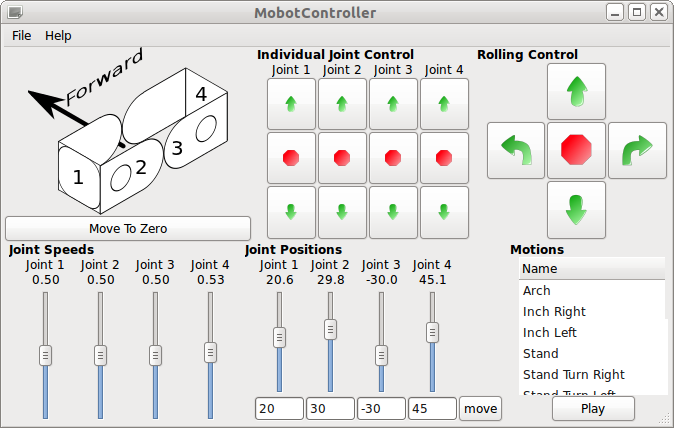
\includegraphics[width=4in]{gui_screenshot.png}
\caption{\label{fig:gui}The iMobot Graphical Control Interface.}
\end{center}
\end{figure}
The iMobot comes with a graphical control interface for controlling the iMobot.
The control interface is able to perform simple locomotion tasks, and can be
used to determine the joint angles of the iMobot. A screenshot of the interface
is shown in Figure \ref{fig:gui}.

The graphical interface can be found in the application menu of the iMobot. Once
a VNC connection to the iMobot has been established, simply left click on the
desktop to bring up the menu, and select the item \texttt{Applications ->
Accessories -> iMobot Controller}. Once the controller starts, it needs to be
initialized in order to establish communication with the motor controllers.
This is done by clicking on \texttt{File -> Init Local I2C Bus}. Ensure that 
the application is connected by ensuring that the status bar at the bottom of the
application displays ``Connected''. 

The graphical interface is composed of four basic components, as shown in
Figure \ref{fig:gui}. The first section, labeled with the red ``1'',
is a section of four sliders. Each slider controls the motor speed of a joint.

The next section, labeled ``2'', are controls which can be used to move each
joint independantly. The upward arrows indicate forward rotation, the stop
buttons stop the motors, and the downward arrows indicate backward motion.
Below the downward arrows are textboxes which display the current angle of each
joint.

The next section, labeled ``3'', contain buttons used for moving the iMobot. 
The arrows indicate forwards and backwards motion, along with turning and
sideways inchworming motions. The large stop sign button stops all motions
on the iMobot. The button labeled ``Home'' causes the iMobot to move all joints
back to their home position. 

The final section, labeled ``4'', contain preprogramed gaits for the iMobot.
To execute a gait, simply select the desired gait by left-clicking on its name,
and click the ``Play'' button.

%%%%%%%%%%%%%%%%%%%%%%%%%%%%%%%%%%%%%%%%%%%%%%%%%%%%%%%%%%%%%%%%%%%%%%
% SUB: Overview of Sample Application Programs {{{
\chapter{Overview of a Sample Application Program}
The following program is a simple program which moves some joints on the iMobot
before initializing the robot to listen for incoming Bluetooth commands.
\subsection{simple.cpp \label{subsec:simple.cpp}}
\listinginput{1}{../Demos/simple_cpp/simple.cpp}
\subsection{Explanation of simple.cpp}
\begin{itemize}
\item Lines 1-3 include the chimobot Ch package. These lines are necessary for
running Ch programs which control the iMobot. 
\item Lines 8-10 declare some local variables that are used throughout the program.
\item Line 10 declares the \texttt{robot} object, which represents the
capabilities of the iMobot module. This object contains various member
functions which may be executed by the user.
\item Lines 13-16 send commands to the iMobot to move all the joints to their
zero position.
\item Line 17 causes the program to wait until all the joints have stopped moving. 
\item Lines 20 and 21 instruct the robot to rotate joints 2 and 3 to rotate 90
degrees. Note that the joint numbers start at 0, so joints 2 and 3 are the
third and fourth joints, respectively. 
\item Lines 23 and 24 cause the program to wait until the third and fourth
joints have stopped moving.
\item Lines 26 and 27 instruct the robot to turn the third and fourth joints
back to their original zero position.
\item Lines 28 and 29 cause the program to wait until the third and fourth
joints have stopped moving.
\item Lines 33 and 34 start the Bluetooth listening service on channel 20,
which listens for Bluetooth remote commands and controls the robot accordingly. 
\item Line 37 terminates the robot control.
\end{itemize}

%%%%%%%%%%%%%%%%%%%%%%%%%%%%%%%%%%%%%%%%%%%%%%%%%%%%%%%%%%%%%%%%%%%%%%
% SUB: Execution of Sample Applications {{{
%\section{Execution of Sample Applications}
%%%%%%%%%%%%%%%%%%%%%%%%%%%%%%%%%%%%%%%%%%%%%%%%%%%%%%%%%%%%%%%%%%%%%%
% Appendix {{{
\appendix
\chapter{libimobot API}
% Mobile-C Library 

%%%%%%%%%%%%%%%%%%%%%%%%%%%%%%%%%%%%%%%%%%%%%%%%%%%%%%%%%%%%%%%%%%%%%%
% Preamble {{{
%\documentclass[11pt]{article}
\documentclass[11pt]{report}
\usepackage{varioref}
\usepackage{times,verbatim,fancyheadings,makeidx}
\usepackage{moreverb}
%\usepackage{psfig}
\usepackage[pdftex]{hyperref}
\usepackage{hypcap}
\usepackage{fullpage}
\usepackage{amssymb,amsmath}
\usepackage{graphicx}
\usepackage{program}
%\headrulewidth 0.0pt
%\hoffset=-0.0625in
%\voffset=0pt
\setlength{\textheight}{9in}
\setlength{\textwidth}{6.5in}
\topmargin=0.05in
\makeindex
% }}} Preamble
%%%%%%%%%%%%%%%%%%%%%%%%%%%%%%%%%%%%%%%%%%%%%%%%%%%%%%%%%%%%%%%%%%%%%%

%%%%%%%%%%%%%%%%%%%%%%%%%%%%%%%%%%%%%%%%%%%%%%%%%%%%%%%%%%%%%%%%%%%%%%
% Title Page {{{
\begin{document}
\thispagestyle{empty}
\begin{center}
%\includegraphics[width=1.8in]{figure/mobilec_logo.png}


\vspace{0.5in}
{\Huge\sf\bf User's Guide for Programming iMobot} \\
\vspace{2.0in}
{\large\sf\bf\today}
%September 20, 2007
\end{center}

\pagebreak
% }}} Title Page
%%%%%%%%%%%%%%%%%%%%%%%%%%%%%%%%%%%%%%%%%%%%%%%%%%%%%%%%%%%%%%%%%%%%%%

%%%%%%%%%%%%%%%%%%%%%%%%%%%%%%%%%%%%%%%%%%%%%%%%%%%%%%%%%%%%%%%%%%%%%%
% Abstract {{{
%\phantomsection
%\addcontentsline{toc}{chapter}{Abstract}
\begin{abstract} 
This library implements control functions for controlling an iMobot
robotic module.

\end{abstract}
\pagebreak
% Abstract }}}
%%%%%%%%%%%%%%%%%%%%%%%%%%%%%%%%%%%%%%%%%%%%%%%%%%%%%%%%%%%%%%%%%%%%%%

%%%%%%%%%%%%%%%%%%%%%%%%%%%%%%%%%%%%%%%%%%%%%%%%%%%%%%%%%%%%%%%%%%%%%%
% Table of Contents {{{
\pagenumbering{roman}
\setcounter{page}{1}
\tableofcontents
\pagebreak
% }}} Table of Contents
%%%%%%%%%%%%%%%%%%%%%%%%%%%%%%%%%%%%%%%%%%%%%%%%%%%%%%%%%%%%%%%%%%%%%%

%%%%%%%%%%%%%%%%%%%%%%%%%%%%%%%%%%%%%%%%%%%%%%%%%%%%%%%%%%%%%%%%%%%%%%
% Part 1 {{{
\pagenumbering{arabic}
\setcounter{page}{1}
\pagebreak
% }}} Part 1 
%%%%%%%%%%%%%%%%%%%%%%%%%%%%%%%%%%%%%%%%%%%%%%%%%%%%%%%%%%%%%%%%%%%%%%

%%%%%%%%%%%%%%%%%%%%%%%%%%%%%%%%%%%%%%%%%%%%%%%%%%%%%%%%%%%%%%%%%%%%%%
% Introduction {{{
%\pagenumbering{arabic}
%\setcounter{page}{1}
%\pagestyle{fancy}
%\chapter{Introduction}
%\pagebreak
% }}} Introduction
%%%%%%%%%%%%%%%%%%%%%%%%%%%%%%%%%%%%%%%%%%%%%%%%%%%%%%%%%%%%%%%%%%%%%%

\chapter{Getting Started}
This short guide will enable you to run the provided demo program,
``simple.cpp'', on the iMobot.
\begin{enumerate}
\item Log in to the imobot. In order to do this, you will need a VNC client. 
  \begin{itemize}
  \item For Windows, you may download and install TightVNC from \texttt{http://www.tightvnc.com}.
  \item For Mac OS X, you may download and install Chicken of the VNC from \texttt{http://sourceforge.net/projects/cotvnc/}.
  \end{itemize}
\item Connect to the iMobot with your VNC client. The default address of the iMobot is \texttt{192.168.0.123}.
\item Copy the demo program to your home directory with the command ``\texttt{cp /usr/local/ch/package/chimobot/demos/simple.cpp ~/}''.
\item Open the demo program with ChIDE. You may left click on the desktop to open the menu, and select \texttt{Applications -> Accessories -> ChIDE}.
\item Click on \texttt{File -> Open} within ChIDE and open the program, \texttt{simple.cpp}. 
\item Click on the ``Run'' button, located near the top right of the ChIDE Window. The robot should now run the program.
\end{enumerate}

\chapter{Gtk iMobot Controller Guide}
\begin{figure}
\begin{center}
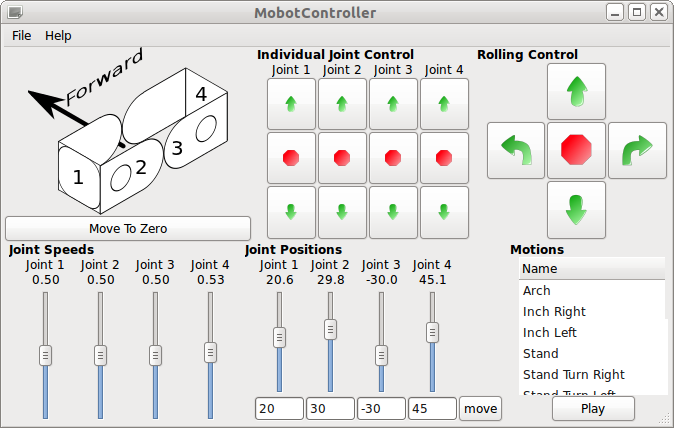
\includegraphics[width=4in]{gui_screenshot.png}
\caption{\label{fig:gui}The iMobot Graphical Control Interface.}
\end{center}
\end{figure}
The iMobot comes with a graphical control interface for controlling the iMobot.
The control interface is able to perform simple locomotion tasks, and can be
used to determine the joint angles of the iMobot. A screenshot of the interface
is shown in Figure \ref{fig:gui}.

The graphical interface can be found in the application menu of the iMobot. Once
a VNC connection to the iMobot has been established, simply left click on the
desktop to bring up the menu, and select the item \texttt{Applications ->
Accessories -> iMobot Controller}. Once the controller starts, it needs to be
initialized in order to establish communication with the motor controllers.
This is done by clicking on \texttt{File -> Init Local I2C Bus}. Ensure that 
the application is connected by ensuring that the status bar at the bottom of the
application displays ``Connected''. 

The graphical interface is composed of four basic components, as shown in
Figure \ref{fig:gui}. The first section, labeled with the red ``1'',
is a section of four sliders. Each slider controls the motor speed of a joint.

The next section, labeled ``2'', are controls which can be used to move each
joint independantly. The upward arrows indicate forward rotation, the stop
buttons stop the motors, and the downward arrows indicate backward motion.
Below the downward arrows are textboxes which display the current angle of each
joint.

The next section, labeled ``3'', contain buttons used for moving the iMobot. 
The arrows indicate forwards and backwards motion, along with turning and
sideways inchworming motions. The large stop sign button stops all motions
on the iMobot. The button labeled ``Home'' causes the iMobot to move all joints
back to their home position. 

The final section, labeled ``4'', contain preprogramed gaits for the iMobot.
To execute a gait, simply select the desired gait by left-clicking on its name,
and click the ``Play'' button.

%%%%%%%%%%%%%%%%%%%%%%%%%%%%%%%%%%%%%%%%%%%%%%%%%%%%%%%%%%%%%%%%%%%%%%
% SUB: Overview of Sample Application Programs {{{
\chapter{Overview of a Sample Application Program}
The following program is a simple program which moves some joints on the iMobot
before initializing the robot to listen for incoming Bluetooth commands.
\subsection{simple.cpp \label{subsec:simple.cpp}}
\listinginput{1}{../Demos/simple_cpp/simple.cpp}
\subsection{Explanation of simple.cpp}
\begin{itemize}
\item Lines 1-3 include the chimobot Ch package. These lines are necessary for
running Ch programs which control the iMobot. 
\item Lines 8-10 declare some local variables that are used throughout the program.
\item Line 10 declares the \texttt{robot} object, which represents the
capabilities of the iMobot module. This object contains various member
functions which may be executed by the user.
\item Lines 13-16 send commands to the iMobot to move all the joints to their
zero position.
\item Line 17 causes the program to wait until all the joints have stopped moving. 
\item Lines 20 and 21 instruct the robot to rotate joints 2 and 3 to rotate 90
degrees. Note that the joint numbers start at 0, so joints 2 and 3 are the
third and fourth joints, respectively. 
\item Lines 23 and 24 cause the program to wait until the third and fourth
joints have stopped moving.
\item Lines 26 and 27 instruct the robot to turn the third and fourth joints
back to their original zero position.
\item Lines 28 and 29 cause the program to wait until the third and fourth
joints have stopped moving.
\item Lines 33 and 34 start the Bluetooth listening service on channel 20,
which listens for Bluetooth remote commands and controls the robot accordingly. 
\item Line 37 terminates the robot control.
\end{itemize}

%%%%%%%%%%%%%%%%%%%%%%%%%%%%%%%%%%%%%%%%%%%%%%%%%%%%%%%%%%%%%%%%%%%%%%
% SUB: Execution of Sample Applications {{{
%\section{Execution of Sample Applications}
%%%%%%%%%%%%%%%%%%%%%%%%%%%%%%%%%%%%%%%%%%%%%%%%%%%%%%%%%%%%%%%%%%%%%%
% Appendix {{{
\appendix
\chapter{libimobot API}
\input{api/libimobot}
\pagebreak
% }}} Appendix 
%%%%%%%%%%%%%%%%%%%%%%%%%%%%%%%%%%%%%%%%%%%%%%%%%%%%%%%%%%%%%%%%%%%%%%

%%%%%%%%%%%%%%%%%%%%%%%%%%%%%%%%%%%%%%%%%%%%%%%%%%%%%%%%%%%%%%%%%%%%%%
% Index {{{
\phantomsection
\addcontentsline{toc}{chapter}{Index}
\printindex
% }}} Index 
%%%%%%%%%%%%%%%%%%%%%%%%%%%%%%%%%%%%%%%%%%%%%%%%%%%%%%%%%%%%%%%%%%%%%%
\end{document}

\pagebreak
% }}} Appendix 
%%%%%%%%%%%%%%%%%%%%%%%%%%%%%%%%%%%%%%%%%%%%%%%%%%%%%%%%%%%%%%%%%%%%%%

%%%%%%%%%%%%%%%%%%%%%%%%%%%%%%%%%%%%%%%%%%%%%%%%%%%%%%%%%%%%%%%%%%%%%%
% Index {{{
\phantomsection
\addcontentsline{toc}{chapter}{Index}
\printindex
% }}} Index 
%%%%%%%%%%%%%%%%%%%%%%%%%%%%%%%%%%%%%%%%%%%%%%%%%%%%%%%%%%%%%%%%%%%%%%
\end{document}

\pagebreak
% }}} Appendix 
%%%%%%%%%%%%%%%%%%%%%%%%%%%%%%%%%%%%%%%%%%%%%%%%%%%%%%%%%%%%%%%%%%%%%%

%%%%%%%%%%%%%%%%%%%%%%%%%%%%%%%%%%%%%%%%%%%%%%%%%%%%%%%%%%%%%%%%%%%%%%
% Index {{{
\phantomsection
\addcontentsline{toc}{chapter}{Index}
\printindex
% }}} Index 
%%%%%%%%%%%%%%%%%%%%%%%%%%%%%%%%%%%%%%%%%%%%%%%%%%%%%%%%%%%%%%%%%%%%%%
\end{document}

\pagebreak
% }}} Appendix 
%%%%%%%%%%%%%%%%%%%%%%%%%%%%%%%%%%%%%%%%%%%%%%%%%%%%%%%%%%%%%%%%%%%%%%

%%%%%%%%%%%%%%%%%%%%%%%%%%%%%%%%%%%%%%%%%%%%%%%%%%%%%%%%%%%%%%%%%%%%%%
% Index {{{
\phantomsection
\addcontentsline{toc}{chapter}{Index}
\printindex
% }}} Index 
%%%%%%%%%%%%%%%%%%%%%%%%%%%%%%%%%%%%%%%%%%%%%%%%%%%%%%%%%%%%%%%%%%%%%%
\end{document}
